%% Two-Sample Test — Conference Presentation
%% Compile: pdflatex main.tex  (run twice for TOC/references)

\documentclass[aspectratio=169, 10pt]{beamer}

% ── Theme ─────────────────────────────────────────────────────────────────────
\usetheme{metropolis}
\setbeamertemplate{frame numbering}[fraction]

% ── Packages ──────────────────────────────────────────────────────────────────
\usepackage{amsmath, amssymb, amsthm}
\usepackage{mathtools}
\usepackage{graphicx}
\usepackage{booktabs}
\usepackage{xcolor}
\usepackage{tikz}
\usepackage{pgfplots}
\pgfplotsset{compat=1.18}
\usepackage{mathrsfs}
\usepackage[style=authoryear, backend=bibtex, maxcitenames=2]{biblatex}
\addbibresource{references.bib}

% ── Notation ──────────────────────────────────────────────────────────────────
%% commands.tex
%% Custom macros and theorem environments for the BNP thesis.

% Draft annotation: \MC{note} renders as coloured inline text
\newcommand{\MC}[1]{\textcolor{red}{\textbf{[MC: #1]}}}

% ============================================================
%  THEOREM ENVIRONMENTS
%  Numbered per section (chapter.section.number).
% ============================================================
% Beamer already defines: theorem, corollary, definition, example, lemma
\theoremstyle{plain}
\newtheorem{proposition}{Proposition}

\theoremstyle{definition}
\newtheorem{assumption}{Assumption}
\newtheorem{remark}{Remark}
\newtheorem{ttheorem}{Tentative Theorem}
\newtheorem*{prop}{Proposition}
\newtheorem*{cor}{Corollary}

% ============================================================
%  Bayesian Nonparametric Toolbox
% ============================================================

% For spaces
\newcommand{\X}{\mathbb{X}}
\newcommand{\Y}{\mathbb{Y}}
\newcommand{\probx}{\mathcal{P}(\mathbb{X})}
\newcommand{\probxtwo}{\mathcal{P}_2(\mathbb{X})}
\newcommand{\probspace}{\left( \Omega, \mathscr{F}, \mathbb{P} \right)}
\newcommand{\probprobx}{\mathcal{P}(\mathcal{P}(\X))}

\newcommand{\lipR}{\mathrm{Lip}_1(\R,\R)}
\newcommand{\lipX}{\mathrm{Lip}_1(\X,\R)}
\newcommand{\lipK}{\mathrm{Lip}_1([-K,K],\R)}
\newcommand{\lipXstar}{\mathrm{Lip}_1^*(\X,\R)}
\newcommand{\lipKzero}{\mathrm{Lip}_1^0([-K,K],\R)}
\newcommand{\dstar}{\D^*}
\newcommand{\ellstar}{\ell^\infty(\dstar)}



\newcommand{\dlip}{d_{\mathrm{Lip}}}
\newcommand{\WW}{\mathcal{W}_{\mathcal{W}}}








% ============================================================
% Some basic notations
% ============================================================
\DeclareMathOperator*{\argmin}{arg\,min}
\newcommand{\R}{\mathbb{R}}
\newcommand{\E}{\mathbb{E}}
\newcommand{\N}{\mathcal{N}}          % Poisson random measure / calligraphic N
\newcommand{\M}{\mathcal{M}}
\newcommand{\G}{\mathcal{G}}
\newcommand{\F}{\mathcal{F}}
\newcommand{\D}{\mathcal{D}}
\newcommand{\W}{\mathcal{W}}
\newcommand{\T}{\mathcal{T}}
\newcommand{\law}{\mathcal{L}}
\newcommand{\var}{\mathrm{Var}}
\newcommand{\cov}{\mathrm{Cov}}
\newcommand{\iid}{\mathrm{i.i.d}}


% ── Title ─────────────────────────────────────────────────────────────────────
\title{Two-Sample Test for Laws of Random Probabilities via \\ Optimal Transport}
\subtitle{The 5th Italian Meeting on Probability and Mathematical Statistics}
\author{{\large George Kanchaveli}}
\institute{Bocconi University}
\date{June 11, 2026}
\titlegraphic{
\includegraphics[height=1.2cm]{figures/Bocconi_University_logo.pdf}}

% ── Custom title page: logo above author, institute below author ───────────────
\setbeamertemplate{title page}{%
  \begin{minipage}[b][\paperheight]{\textwidth}%
    \vfill
    {\usebeamerfont{title}\usebeamercolor[fg]{title}\inserttitle\par}%
    \vfill
    \inserttitlegraphic\par%
    \vspace{0.6em}%
    {\usebeamerfont{author}\usebeamercolor[fg]{author}\insertauthor\par}%
    \vspace{0.3em}%
    {\usebeamerfont{institute}\usebeamercolor[fg]{institute}\insertinstitute\par}%
    \vfill
    {\usebeamerfont{subtitle}\usebeamercolor[fg]{subtitle}\insertsubtitle\par}%
    \vspace{0.3em}%
    {\usebeamerfont{date}\usebeamercolor[fg]{date}\insertdate\par}%
    \vspace{1em}%
  \end{minipage}%
}

% ─────────────────────────────────────────────────────────────────────────────
\begin{document}

\maketitle

% ── Joint work slide ──────────────────────────────────────────────────────────
\begin{frame}[c]
  \begin{center}
    {\large\bfseries Joint work with}
  \end{center}
  \vspace{1.5em}
  \begin{columns}[c]
    \begin{column}{0.45\textwidth}
      \begin{center}
        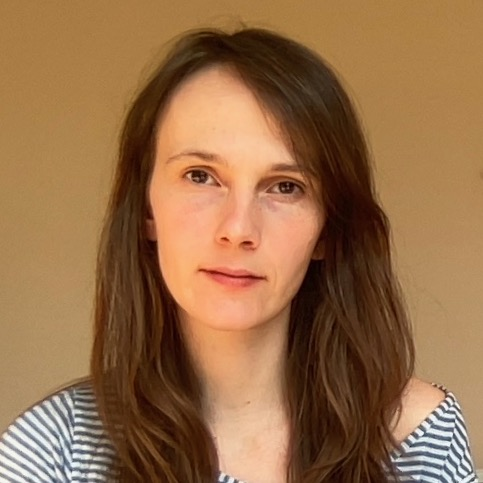
\includegraphics[height=3.5cm, keepaspectratio]{figures/martacatalano.jpeg}\\[0.4em]
        {\bfseries Marta Catalano}\\[0.5em]
        
\includegraphics[height=1cm]{figures/luissuniversity_logo.jpeg}
      \end{center}
    \end{column}
    \begin{column}{0.45\textwidth}
      \begin{center}
        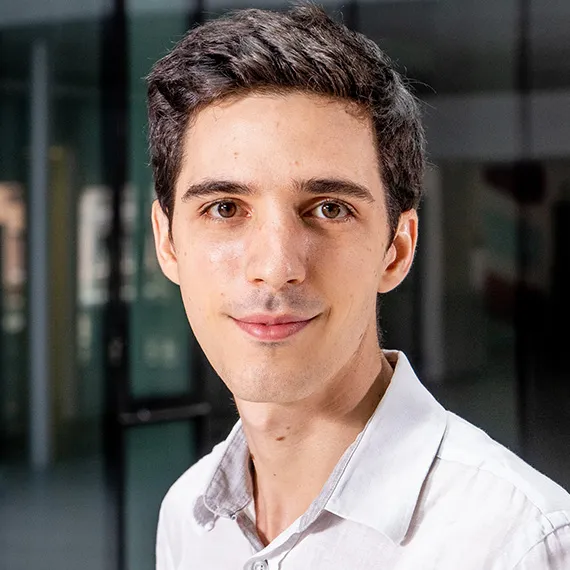
\includegraphics[height=3.5cm, keepaspectratio]{figures/hugolavenant.png}\\[0.4em]
        {\bfseries Hugo Lavenant}\\[0.5em]
        
\includegraphics[height=1cm]{figures/Bocconi_University_logo.pdf}
      \end{center}
    \end{column}
  \end{columns}
\end{frame}

\begin{frame}{Outline}
  \tableofcontents
\end{frame}

% =============================================================================
\section{Motivation}
% =============================================================================

\begin{frame}{Frame Title}
  % content
\end{frame}

% =============================================================================
\section{Method}
% =============================================================================

\begin{frame}{Frame Title}
  % content
\end{frame}

% =============================================================================
\section{Theory}
% =============================================================================

\begin{frame}{Frame Title}
  % content
\end{frame}

% =============================================================================
\section{Simulations}
% =============================================================================

\begin{frame}{Frame Title}
  % content
\end{frame}

% =============================================================================
\section{Conclusion}
% =============================================================================

\begin{frame}{Frame Title}
  % content
\end{frame}

\begin{frame}{References}
  \printbibliography[heading=none]
\end{frame}

% ── Appendix ──────────────────────────────────────────────────────────────────
\appendix

\begin{frame}{Backup Slide}
  % content
\end{frame}

\end{document}